% Chapter 2

\chapter{Research Methodology} % Write in your own chapter title
\label{Chapter 4}
\lhead{Chapter 4. \emph{Research Methodology }} % Write in your own chapter title to set the page header

\section{Introduction}
After the literature review, we conclude that the most of the applications are based on outdoor localization such as GPS. This application only tells the outdoor locations on the maps. When we are out of the building, it’s only shows the boundaries of the buildings not the rooms. But we want to create an application which tells about the indoor location. This application is based on room level prediction. It’s not only tells the room level prediction but also tells the entire information of the room. 
\\
The purpose of writing this chapter is to explain the methodology for making this indoor localization based application. We want to tell that which methods and approaches we used to develop this application. We will also explain that which ML (Machine Learning) algorithms are used, how to collect the data, how to analyze data for this application. We also describe the use cases, use case diagram and test cases of this application. 

\section{Research Methodology}
From the literature review, we conclude that the concept of outdoor localization is introduced on the behalf of GPS. People can access anywhere when he is on the GPS which is installed on every smart phone. But people can only see the boundaries of the building not the rooms of the buildings. They did not know the entire information of the building. They do not know the concept of indoor localization. People face the problem to know the entire information of the building. For example, when a student enters the University for Admission, he/she did not know the ways of the university. They have to face the problem where is Admin block? Where is library? Where is department? Furthermore, if people enter to the hospital, offices, buildings etc., than they did not know the indoor location of those places.  To answer all of these questions, we want to develop the application which tells the indoor location of the building. It not only tells the room name but also tells the entire information of the room. If we talk about the building of the university, then it also tells us the room member name, its office hours etc. We provide this information in the form of texture, audios and pictures.
\\\\
\section{Proposed Work to develop the Android Application}
Actually, we cannot refuse that many indoor applications also developed but they all used different technologies. Most of the indoor applications used Wi-Fi for predict the position of the person that tells the indoor location of that person. But we have to develop the system which tells the indoor location of the person which is based on BLE beacons. BLE beacon is the Bluetooth device which consumes less energy. It is light weight and cheaper than Wi-Fi signals. BLE beacons are usually battery powered, which are more flexible. It is easier to sense the signals. 
We don’t have enough resources to make this application globally. Now, we make this application for our computer Engineering department, UET. To develop this system, we consider the number of points which tells the methods to develop the system that is as follows:
\begin{itemize}
\item First of all, we deploy the BLE beacons in our department. BLE beacons will be installed on the ceilings of rooms.
\item We capture the RSSI fingerprints of BLE beacons at different position using data capturing. By using this application .csv file will be generated. 
\item Data will be pre-processed and trained by using machine learning algorithm such as KNN, ANN and random forest.
\item After capturing and train the data, we integrate the data with our android application. For this purpose, we made two android applications. One is admin application and the other is user application.
\item We made the android admin app to add, edit and delete the data of rooms. We can also add, edit and delete the data of room members. Also, we can add, edit, delete office hours of the room members. We can also add pictures and audio of the room
\item At the end, we made the android user application. First of all, we integrate the data using different API. We need to make the API to integrate the data.
\item  After integration of data, when user reach the room of our department, he/she can see the details of rooms, room members and also see the details of  office hours of the room members in the form of texture, audios and pictures.
\end{itemize}
\section{Related Work}
Different Indoor applications are exit. But their functionality is different. One of the indoor applications is Image based indoor localization. The data set of this application is images, image features and annotations. Some of the images features are SIFT, PCA-SIFT and SURF.  For capture the image, we have to use omni directional camera. It consists of three wheels tripod stand. But we capture the image from the laptop. System easily covered the wide area. After capture the image, the location of the image is also stored by using the interface. The annotation data consists of (x, y, z) coordinates. It also has the information of room name, floor and show case name for the image. 
For this Image based indoor localization, they use fast nearest neighbor algorithm that is ANN and LSH (Locality- Sensitive-Hashing). LSH is the nearest neighbor search technique which uses the hash function. It is noticed that LSH is the faster than other algorithms.
Here are the some experimental results of this Image based indoor localization. By applying these algorithms, it shows the precision and processing time of each feature.


\begin{figure}[h]
  		\centering
    		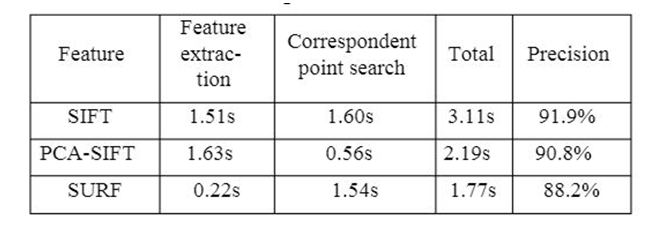
\includegraphics[scale=0.8]{./Figures/feature}
\caption{Precision and processing time of features}
\label{fig:1}
 		\end{figure}

Now we discuss about another application of capacitive sensors based on indoor localization. Capacitive sensing is that technique that tracking the conductive and non-conductive objects. This sensor is able to sense the 3D position of human and their interacting objects. 
 By using this technique, we can find the indoor location of the person by using human-body detection technique. It uses capacitive transducers which operate in 3 modes. But in this case, we use only 2 modes known as shunt mode or transmit mode for the detection of the body. Another scientist introduced the load operation mode. In this mode, human body acts as a potential-plate that is shown in Fig (a). Capacitances used in load mode are Cpb (plate-body capacitor), Cbg (body-ground capacitor) and Cpg (plate-ground capacitor). It is more suitable for deployment. For develop capacitive sensors based application, load operation mode is used.


\begin{figure}[h]
  		\centering
    		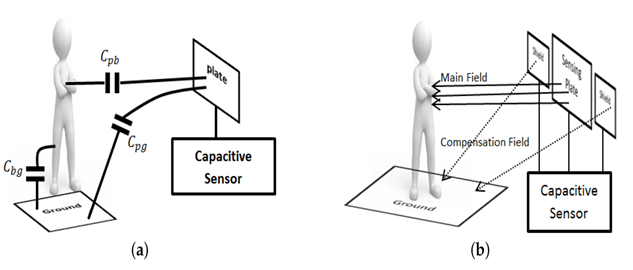
\includegraphics[scale=0.8]{./Figures/systemarchi}
\caption{System Architecture}
\label{fig:2}
 		\end{figure}
For develop this system, they also use some algorithms such K-NN (K-Nearest Neighbor), NB (Naive Byes), SVM (Support Vector Machine). To perform the experiment, they have a room in which they place sensor plates of 4cmX4cm. They deploy the sensors on the four sides of the room. After deploy the sensors, they used three algorithms as we explain above. These algorithms used to find the precision and recall of this indoor localization system. The precision and recall are given in table below:   

\begin{figure}[h]
  		\centering
    		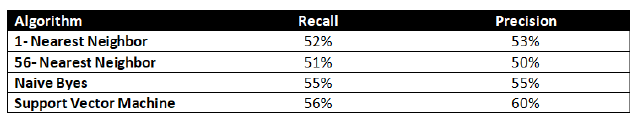
\includegraphics[scale=0.9]{./Figures/pr1}
\caption{Precision and recall of different algorithms}
\label{fig:3}
 		\end{figure}

They also perform this experiment with the room having sensor plates of 8cmX8cm. The results of precision and recall are different from the above results. They give better result than the above. The precision and recall of 8cmX8cm sensor plates are given in table below:  

\begin{figure}[h]
  		\centering
    		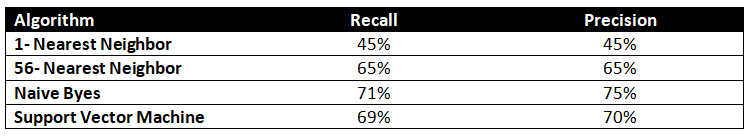
\includegraphics[scale=0.75]{./Figures/pr2}
\caption{Precision and recall of different algorithms}
\label{fig:4}
 		\end{figure}

They also perform this experiment with the room having sensor plates of 16cmX16cm. The results of precision and recall are also different from the above results. They give best result than all of the above. The precision and recall of 16cmX16cm sensor plates are given in table below:  

\begin{figure}[h]
  		\centering
    		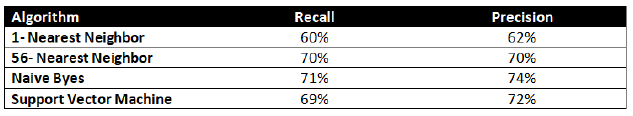
\includegraphics[scale=0.9]{./Figures/pr3}
\caption{Precision and recall of different algorithms}
\label{fig:5}
 		\end{figure}
Another most important technology, we discuss here. We have to discuss the indoor based localization using Wi-Fi. This application also tells the user to the position of the person where he stands. It also tells the indoor localization of the person. The patterns that connect the different access point of the Wi-Fi which is fixed to the various point and become unique. This pattern is called Wi-Fi finger printing. It consists of Received Signal Strength Indicator (RSSI) values and MAC Address data. RSSI values contain negative numbers. If RSSI values are closest to the zero (0) such as (-5) then It indicates that the signal strength is strong. 
The data set of this application consists of RSSI value and MAC address. The algorithms of machine learning also apply in this indoor based localization using Wi-Fi application. Due to the large data set. The fastest algorithm is used in this system. The algorithm which is used in this application is deep learning. Meanwhile, the machine learning algorithms such as k-NN, NB, SVM also used for this application. Their precision and recall also shown in table:

\begin{figure}[h]
  		\centering
    		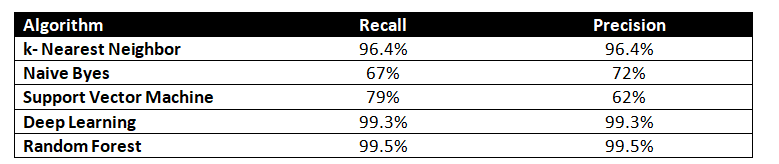
\includegraphics[scale=0.7]{./Figures/pr4}
\caption{Precision and recall of different algorithms}
\label{fig:6}
 		\end{figure}


\subsection{Comparison of Existing Work}
Here are the comparisons of some of them
\begin{figure}[h]
  		\centering
    		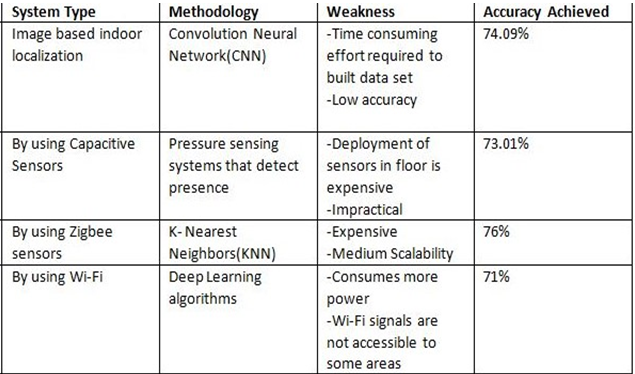
\includegraphics[scale=0.9]{./Figures/comparison}
\caption{Comparison between existing systems}
\label{fig:7}
 		\end{figure}

\subsection{Limitations of Existing System}
Here are some limitations of existing system which are as follows:
\begin{itemize}
\item In some systems, camera is required for indoor positioning which is not suitable for some users.
\item High cost and effort is required for the deployment of indoor localization.
\item Most of the existing systems have medium or low accuracy.
\item In image based indoor localization, time consuming effort is required for built data sets. 
\item It consumes more power.
\item There are some spots where Wi-Fi access points would be difficult to access.
\\\\
\end{itemize}

\subsection{Software Architecture}
Here is our software architecture:
\\\\
\begin{figure}[h]
  		\centering
    		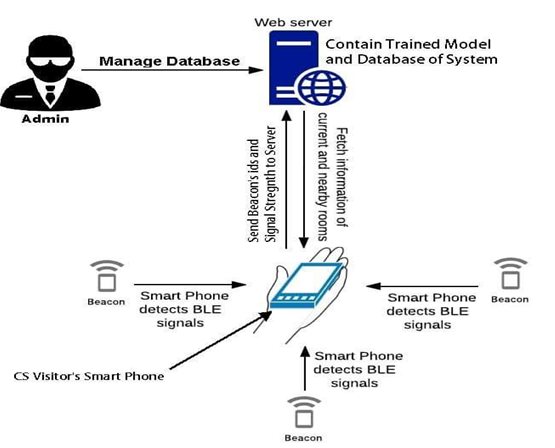
\includegraphics[scale=0.9]{./Figures/softarchi}
\caption{Software Architecture Diagram}
\label{fig:8}
 		\end{figure}


\section{Software Development Life Cycle Used}
To implement a project, one must have to follow some software development life cycle to deliver his project completely according to user requirements in time. By following a certain SDLC, a project developer feels so comfortable as he have specific tasks and time to implement project timely  which meets the user’s point of view. In our project, there are lots of fluctuations time by time. So, we decided to follow AGILE model.
\subsection{AGILE SDLC}
Agile SDLC model is a combination of incremental and iterative process models deals with customer requirements satisfaction and process adaptability by rapid delivery of working product to the customer. This model breaks the whole project in small modules. Do proper testing after completion of each module. Then deliver this working module to the customer and important stakeholders to satisfy them. If that module doesn’t meet their point of views properly or to which customer point of view as he didn’t explained in the document, then it has to be iterated to fulfill their new recommendations. And the other perspective is that if the customer wants to add some functionality in that particular module then a developer has to follow an incremental technique to add specific functionalities. 
To complete each deliverable module of the project, developer has to follow these steps
\begin{itemize}
\item Planning
\item Requirements Analysis
\item Design
\item Coding
\item Unit Testing and
\item Acceptance Testing
\end{itemize}

\begin{figure}[h]
\begin{center}
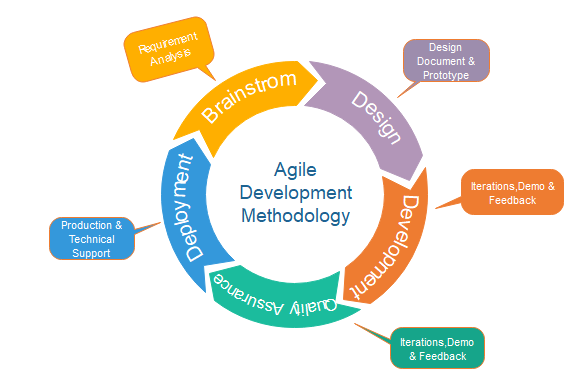
\includegraphics[scale=0.6]{agile}
\caption{Agile Development Methodology}
\label{fig:9}
\end{center}
\end{figure}
\subsection{Justification for AGILE SDLC}

These steps will justify that our project is based on agile methodology:
\begin{itemize}
\item All the requirement specifications and the scope of the project is strictly defined in our documentation but by the time, it may require some amendments, so they will change by ourselves.
\item Planning of time, design, implementation and testing is done.
\item Hardware and software parts of our project are specified into a work breakdown structure.
\item All the Modules of our project are divided in small pieces of time according to estimated time.
\item In model training module, we first use Weka and then following TensorFlow to meet the requirements; hence we followed an incremental and iterative model.
\item Do unit and acceptance testing after completion of each module.
\item Budget plan for our project is defined
\item We Add functionality of delay in Data Capturing application  which capture data after some seconds when a user change his indoor location.
\item Add restart functionality to restart scanning of Bluetooth devices once it stops which leads to incremental change in data capturing application.
\item Roles and responsibilities of team members vary according to the prescribed task and time limit.
\end{itemize}


\section{Requirement Analysis}
The most important section of system requirement specification document is requirement analysis. To start any project, anyone needs to know his system requirements. This section includes all the software, hardware functional requirements of our system, user interfaces, database diagram, use case diagram, use case tests and test cases. Basically, we will discuss all the specifications of our system.
\subsection{Hardware Functional Requirements}
\textbf{Deployment of BLE beacons}

Deployment of BLE beacons on the ceiling is the requirement to capture fingerprints of BLE beacons with different mobile devices. At what angle and at what part of the ceiling these beacons should display, all we get it know before their deployment.

\subsection{Software Functional Requirements}
\subsubsection{Data Capturing Application}
\textbf{Bluetooth scanning for nearby devices}

A scanning function is made in data capturing application to scan BLE beacon for nearby mobile devices. Devices who present/locate near a certain BLE beacon are being scanned.

\textbf{Capture RSSI values for nearby beacons}
BLE beacons Bluetooth range exists in a certain region and this region contain different mobile devices far and near to BLE beacon depending upon their indoor location. So, this function will capture RSSI fingerprints for all mobile devices which being scanned in that certain region.

\textbf{Add delay factor to capture FP’s}
 
Once fingerprints of certain mobile device have been captured at a particular location and by determining the indoor location, we provide room information through our application to a user’s mobile device. The user may change his indoor location after a while. To provide updated room information to the user we are making a delay function which captures user fingerprints after a certain time (seconds) and provide him updated information according to his room location.

\textbf{Automatic restart Bluetooth scanning for nearby devices once it stops}
 
Automatic restart scanning function will scan for BLE beacon nearby mobile devices once scanning has been stops, because in this way our system will able to automatically find coming and going devices in a particular region and provide rooms information accordingly.

\textbf{Generate .csv file for each BLE beacon}
 
After capturing the fingerprints of all devices with a single BLE beacon which lie in that certain region, this function will generate .csv file and RSSI values of all devices in that file.


\textbf{\textbf{\subsubsection{SmartGuide: Android Application}}}

The functional requirements of our system for User are as follows:

\textbf{Load trained model in Android app}

There is need to load machine learning trained model in our Android application to predict the room location of a particular person.

\textbf{Get the prediction of room from trained model}

When a trained model receives .csv file of a particular BLE beacon, it gives the particular roomID of that beacon to a mobile device which is receiving higher RSSI value from that BLE beacon.

\textbf{Allow user to know his indoor location}

This function will enable users to see their indoor location i.e. in which room they are.

\textbf{Fetch information of that particular room}

This function will send RoomID of a particular BLE beacon to the database from which room information in image, texts and audio format can be fetched.

\textbf{Provide information of the room to the user}

After fetching the information of a particular room, this function becomes enable and displayed that information on user mobile screen.

\textbf{Enable user to get information of nearby rooms}

This function allow users to see their nearby (left, right, front and back) rooms and textual and pictorial information about that rooms.
\\\\
The functional requirements of our system for Admin are as follows:

\textbf{Allow admin to SignUp for our application}

To use an Android application, in this case admin has to register on our application to add, update and delete records of certain data in our application.

\textbf{Provide account activation functionality to the admin}

Admin can login on another device; he has no restriction to use our application on a certain device. He may be login or logged out.

\textbf{Admin has all the records of data}

Admin has the ability to get all up-to-date records of data. Data can be of staff members, their visiting hours, room information, lab accessories and much more.

\textbf{Store information to database in images, audios and text format of rooms and their nearby rooms}

This function will store information about rooms in images, audios and text format in the database. Also, the information about nearby rooms of a certain room will also be stored by the admin in the database manually.

\textbf{Allow admin to edit or update the information about rooms}

When After sometime, the specifications and in formations about certain rooms and departments can be changed. So, this function will enable admin to update the information accordingly to provide up-to-date information to the user.

\textbf{Admin has all those functionalities which a user has}

Admin can see the information of a room and nearby rooms in any format provided in our application like user.

\subsection{Non Functional Requirements}
\textbf{Reliability}

Our project will be reliable .The user’s information will be kept confidential and there will be no worry of losing the information.

\textbf{Usability}

Our application will be usable for the users and easy to use.

\textbf{Maintainability}

This system will have the capability to adapt changes and amendments done in the database by the admin as the information of rooms will be updated or edited.

\textbf{Security}

Our Android application will work under potential risks. It will not be accessible by the malicious user or be crashed by external attacks.

\textbf{Recoverability}

In case of crash, our system information will recoverable

\textbf{Safety}

Optimize safety in the design, development, use and maintainability of the application.

\textbf{Reusability}

Our system will provide reusability factor to the visitors of the department.

\textbf{Performance}

To make a system which gives accurate and up-to-date information about rooms even a user change his indoor location after a while. This system will give results efficiently in small time.


\subsection{Use Case Diagram}
\begin{figure}[h]
\begin{center}
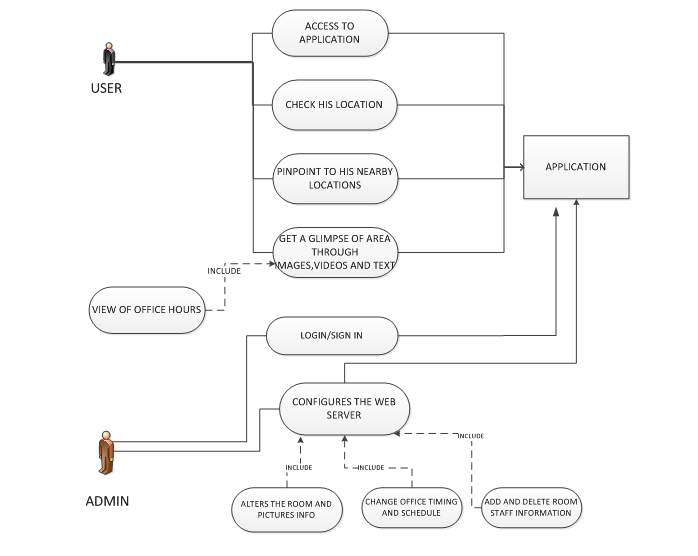
\includegraphics[scale=1.0]{usecase}
\caption{Usecase Diagram}
\label{fig:10}
\end{center}
\end{figure}
\clearpage
\subsection{Use Case Texts}

\begin{figure}[h]
\begin{center}
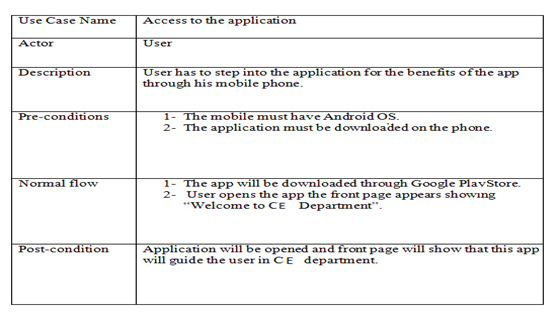
\includegraphics[scale=0.8]{uc1}
\caption{Usecase(1)}
\label{fig:11}
\end{center}
\end{figure}


\begin{figure}[h]
\begin{center}
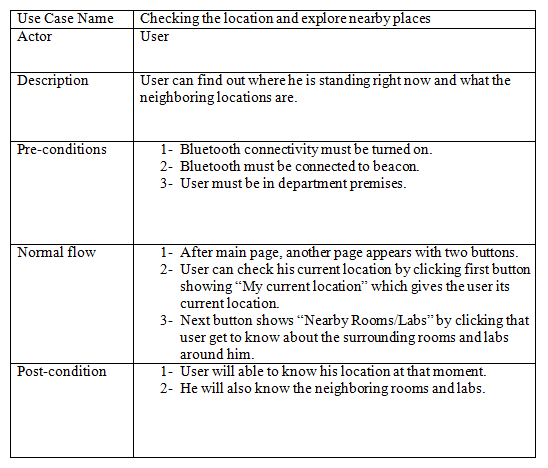
\includegraphics[scale=0.8]{uc2}
\caption{Usecase(2)}
\label{fig:12}
\end{center}
\end{figure}

\begin{figure}[h]
\begin{center}
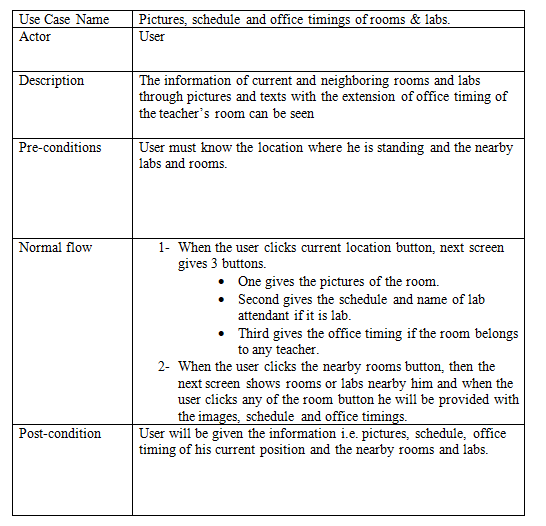
\includegraphics[scale=0.8]{uc3}
\caption{Usecase(3)}
\label{fig:13}
\end{center}

\end{figure}

\begin{figure}[h]
\begin{center}
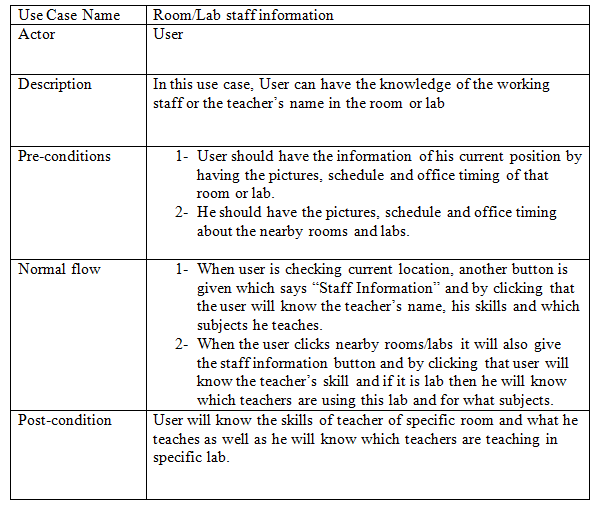
\includegraphics[scale=0.7]{uc4}
\caption{Usecase(4)}
\label{fig:14}
\end{center}
\end{figure}

\begin{figure}[h]
\begin{center}
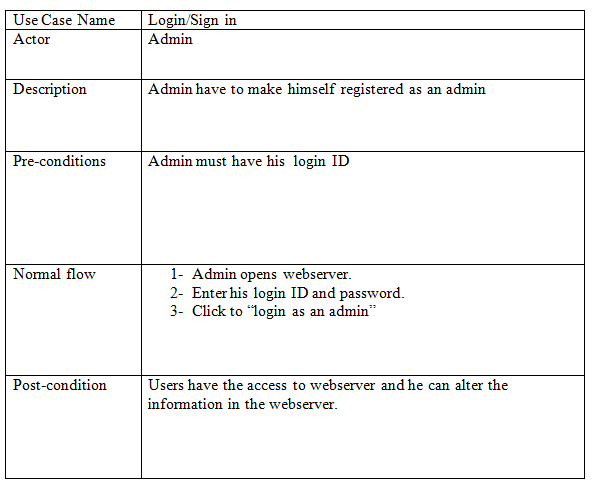
\includegraphics[scale=0.77]{uc5}
\caption{Usecase(5)}
\label{fig:15}
\end{center}
\end{figure}

\begin{figure}[h]
\begin{center}
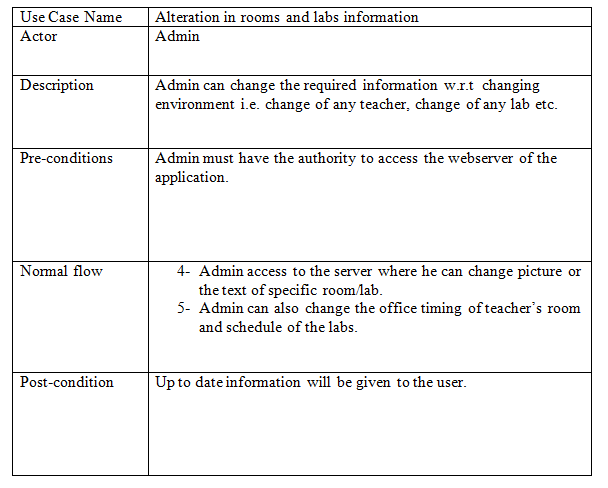
\includegraphics[scale=0.75]{uc6}
\caption{Usecase(6)}
\label{fig:16}
\end{center}
\end{figure}

\begin{figure}[h]
\begin{center}
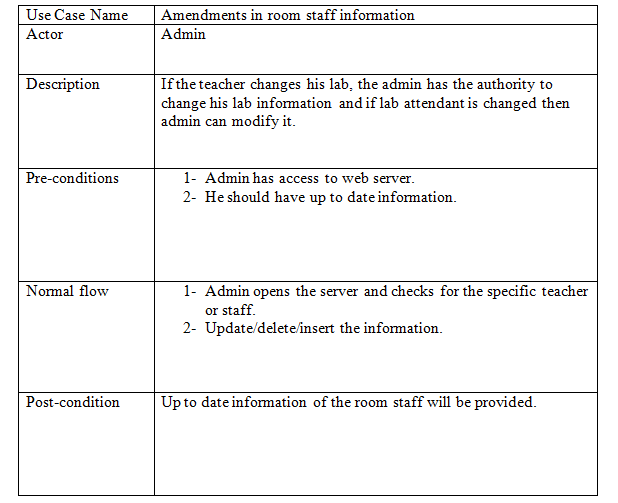
\includegraphics[scale=0.75]{uc7}
\caption{Usecase(7)}
\label{fig:17}
\end{center}
\end{figure}

\begin{figure}[h]
\subsection{Test Cases}
\begin{center}
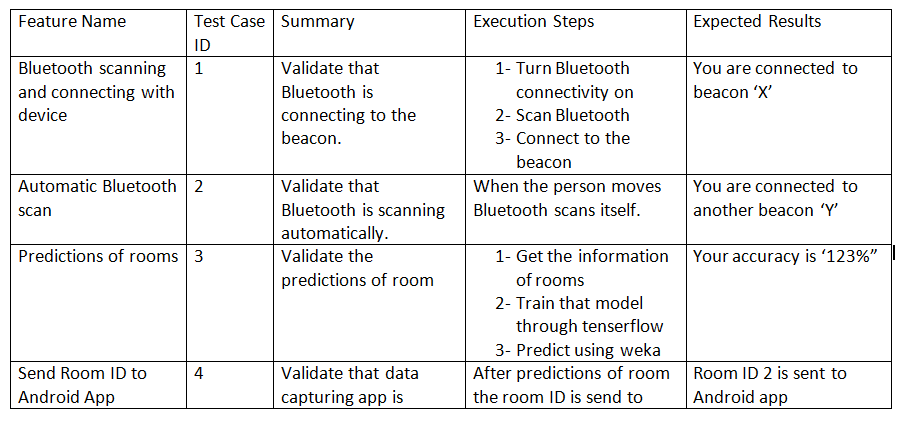
\includegraphics[scale=0.7]{tc1}
\caption{Testcase(1)}
\label{fig:18}
\end{center}
\end{figure}

\begin{figure}[h]
\begin{center}
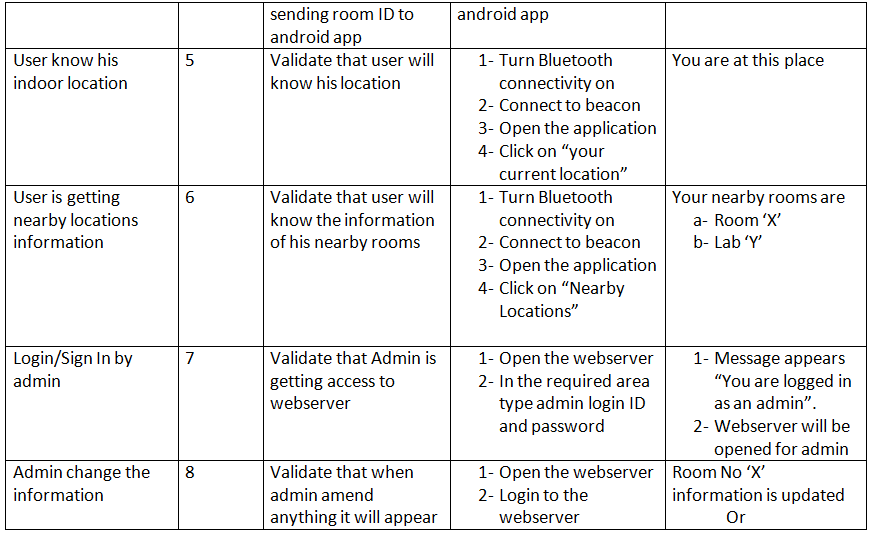
\includegraphics[scale=0.7]{tc2}
\caption{Testcase(2a)}
\label{fig:19}
\end{center}
\end{figure}

\begin{figure}[h]
\begin{center}
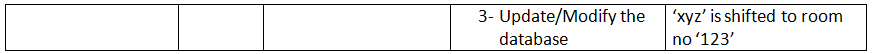
\includegraphics[scale=0.7]{tc3}
\caption{Testcase(2a)}
\label{fig:20}
\end{center}
\end{figure}


\clearpage


\section{Proposed System}

In our proposed system, an Android application provide guidance to campus isitors and make them familiar with department. Application will not only tell the current indoor location of user but also the information about current indoor location and nearby rooms in textual, image and audio formats. The location of the user is determined by taking predictions from the trained machine learning model on specific dataset. Dataset contains the RSSI fingerprints of BLE beacons  which we installed in the department, their MAC addressess and room rabels which we assigned to each room of the department in order to predict the class label. This dataset captured through a seperate Android Application named (BLE Scanner RSSI) which captures the RSSI values of nearby beacons from mobile device. 
Basically, there are two Android Applications, one is for the user through which we guide the user about the department through pictorial and textual information and the other application is for the admin who can do ammendments in the database. The database contains the information about rooms of the department i.e. the schedule of each lab for each class or the visiting hours and the specifcations of particular teacher and staff members. Semesterwise schedules, timetables and lab attendees varies timely in the department so this was must to update the information accordingly.
\\

\begin{figure}[h]
\begin{center}
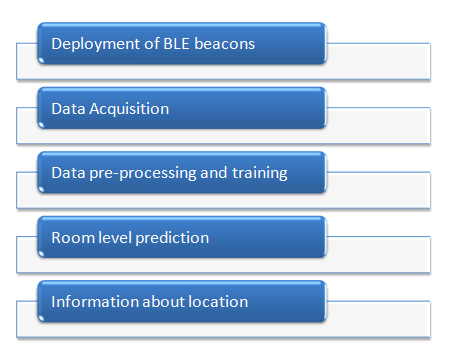
\includegraphics[scale=0.8]{proposedsystem}
\caption{Proposed System}
\label{fig:21}
\end{center}
\end{figure}

\clearpage
 \subsection{Deployment of BLE Beacons}
BLE beacons deployed in the experimental area which is Computer Engineering department of UET, Lahore. All the rooms of experimental area are assigned with a specific class label through which predict the location of the user's mobile device.Each room has its own lable range from L1 to L23. The detailed descritpion of the installment of BLE beacons in each room and floor of experimental area is shown in the figure below:

\begin{figure}[h]
\begin{center}
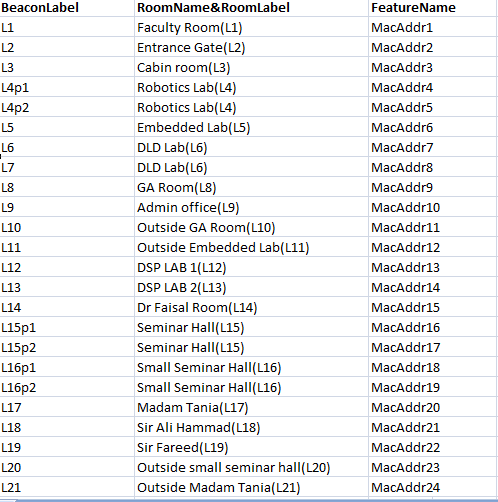
\includegraphics[scale=0.8]{beaconlabel}
\caption{Beacons labeling}
\label{fig:22}
\end{center}
\end{figure}

The placement of BLE beacons in the rooms, labs, corridors of both floors of the department is shown in previous chapter in detail.
\\

 \subsection{Data Acquisition}
BLE beacons broadcasts signals and these signals in the form of RSSI values will be captured at different positions by using Android application named(BLE Scanner RSSI) and then csv file will be generated which contains the MAC addresses of nearby BLE beacons from mobile device, class label and the RSSI fingerprints in the form of numerical values.

\begin{figure}
\begin{center}
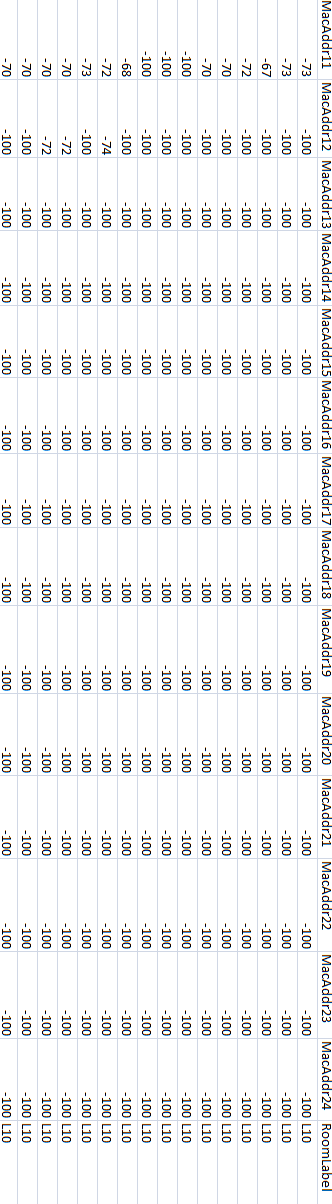
\includegraphics[scale=0.8]{dataeg}
\caption{Small portion of dataset}
\label{fig:23}
\end{center}
\end{figure}

\clearpage
 \subsection{Data Pre-processing and Training}
Pre-processing is done by replacing the null values of dataset by minimum signal strenth a device can recieve from BLE beacon according to our datset which is -100.Also, it includes the concatenation of thousand of csv files in one csv file to place our dataset at one place in file. Then this file is being used as an input to training algorithm, on which a classifier trains its model and make predictions. We trained this dataset by using machine learning algorithms i.e. knn, ann, random forest but artificial neural network gives us the high accuracy of training model as shown in figure. So, we decide to use ann as our selecetd model  and deployed this model on server.So, we can integrate our model to our Android application. 


\subsection{Room Level Prediction}
An Android application for common users will be developed that capture RSSI signals and send to server. Then trained model will take these values as input for the purpose of prediction of room and then send back the room label and its information to the user's application.
\subsection{Location Information}
Application will fetch information data of current room and nearby rooms in bith textual and pictorial formats from server and then display this information on the screen.







